\documentclass{standalone}
\usepackage{tikz}
\usepackage{pgf-umlcd}
\usepackage{fontspec,xcolor,ifthen,xifthen}

\setmonofont[
    AutoFakeSlant,
    BoldItalicFeatures={FakeSlant},
]{Inconsolatazi4}

\newcommand{\fieldType}[2]{\texttt{\color{red}{#1:\hspace{1mm}#2}}}
\newcommand{\funcType}[4][]{\texttt{\color{blue}{#2(#3)%
    \ifthenelse{\isempty{#4}}%
    {}%
    {\hspace{1mm}#4}%
    \ifthenelse{\isempty{#1}}%
    {}%
    {:\hspace{1mm}#1}%
}}}

\begin{document}

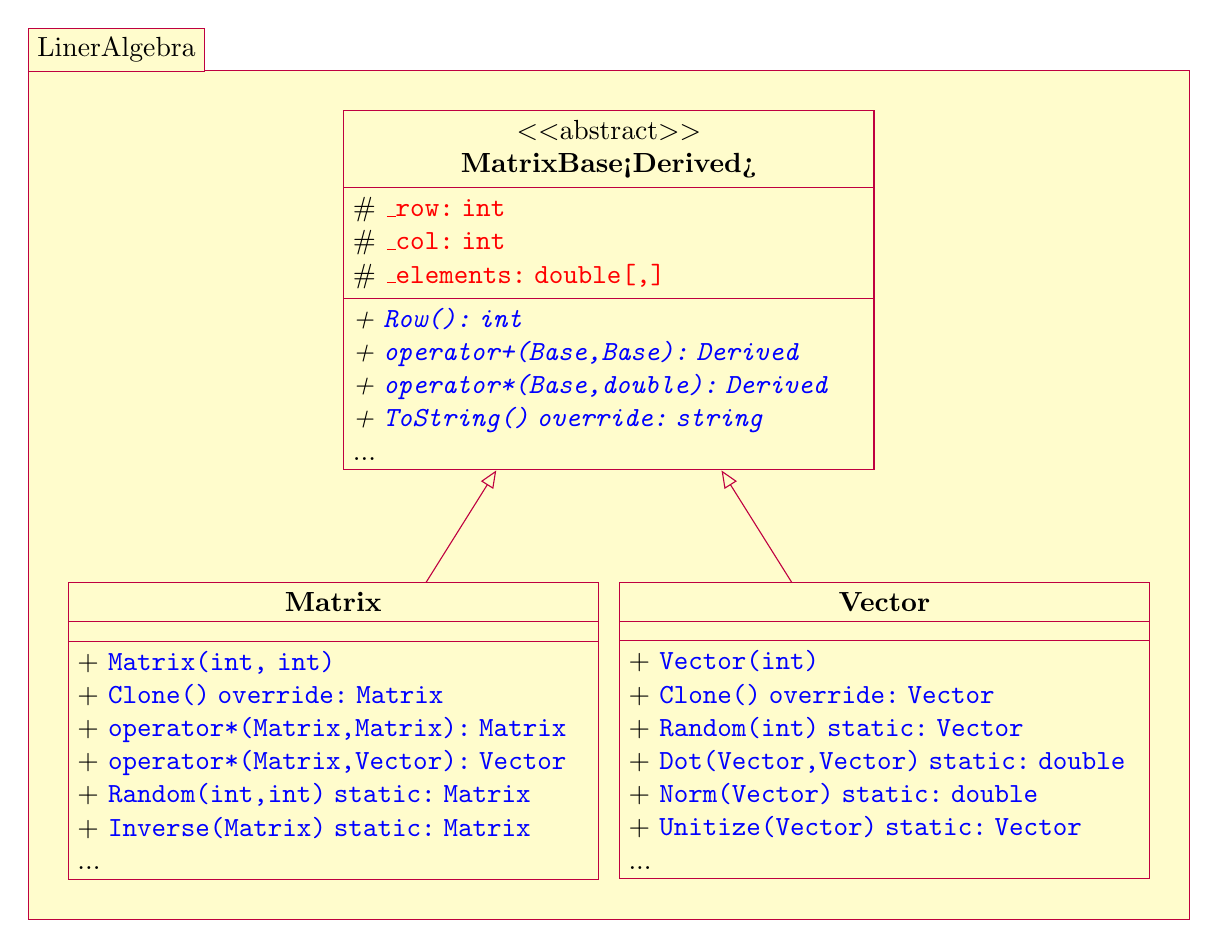
\begin{tikzpicture}
\begin{package}{LinerAlgebra}
\begin{abstractclass}[text width =6.5 cm]{MatrixBase<Derived>}{0 ,1}
\attribute{\# \fieldType{\_row}{int}}
\attribute{\# \fieldType{\_col}{int}}
\attribute{\# \fieldType{\_elements}{double[,]}}
\operation[0]{+ \funcType[int]{Row}{}{}}
\operation[0]{+ \funcType[Derived]{operator+}{Base,Base}{}}
\operation[0]{+ \funcType[Derived]{operator*}{Base,double}{}}
\operation[0]{+ \funcType[string]{ToString}{}{override}}
\operation{...}
\end{abstractclass}
\begin{class}[text width =6.5cm]{Matrix}{-3.5 , -5}
\inherit{MatrixBase<Derived>}
\operation{+ \funcType{Matrix}{int, int}{}}
\operation{+ \funcType[Matrix]{Clone}{}{override}}
\operation{+ \funcType[Matrix]{operator*}{Matrix,Matrix}{}}
\operation{+ \funcType[Vector]{operator*}{Matrix,Vector}{}}
\operation{+ \funcType[Matrix]{Random}{int,int}{static}}
\operation{+ \funcType[Matrix]{Inverse}{Matrix}{static}}
\operation{...}
\end{class}
\begin{class}[text width =6.5 cm]{Vector}{3.5 , -5}
\inherit{MatrixBase<Derived>}
\operation{+ \funcType{Vector}{int}{}}
\operation{+ \funcType[Vector]{Clone}{}{override}}
\operation{+ \funcType[Vector]{Random}{int}{static}}
\operation{+ \funcType[double]{Dot}{Vector,Vector}{static}}
\operation{+ \funcType[double]{Norm}{Vector}{static}}
\operation{+ \funcType[Vector]{Unitize}{Vector}{static}}
\operation{...}
\end{class}
\end{package}
\end{tikzpicture}

\end{document}